% Detailed publication captions for the five validation panels of
% the Finite-Agent Coordination manuscript.
% Each caption describes axes, ranges, scales, the theoretical formula,
% the relevant theorem reference, and the measured precision against
% the closed-form prediction.

\begin{figure*}[!htbp]
    \centering
    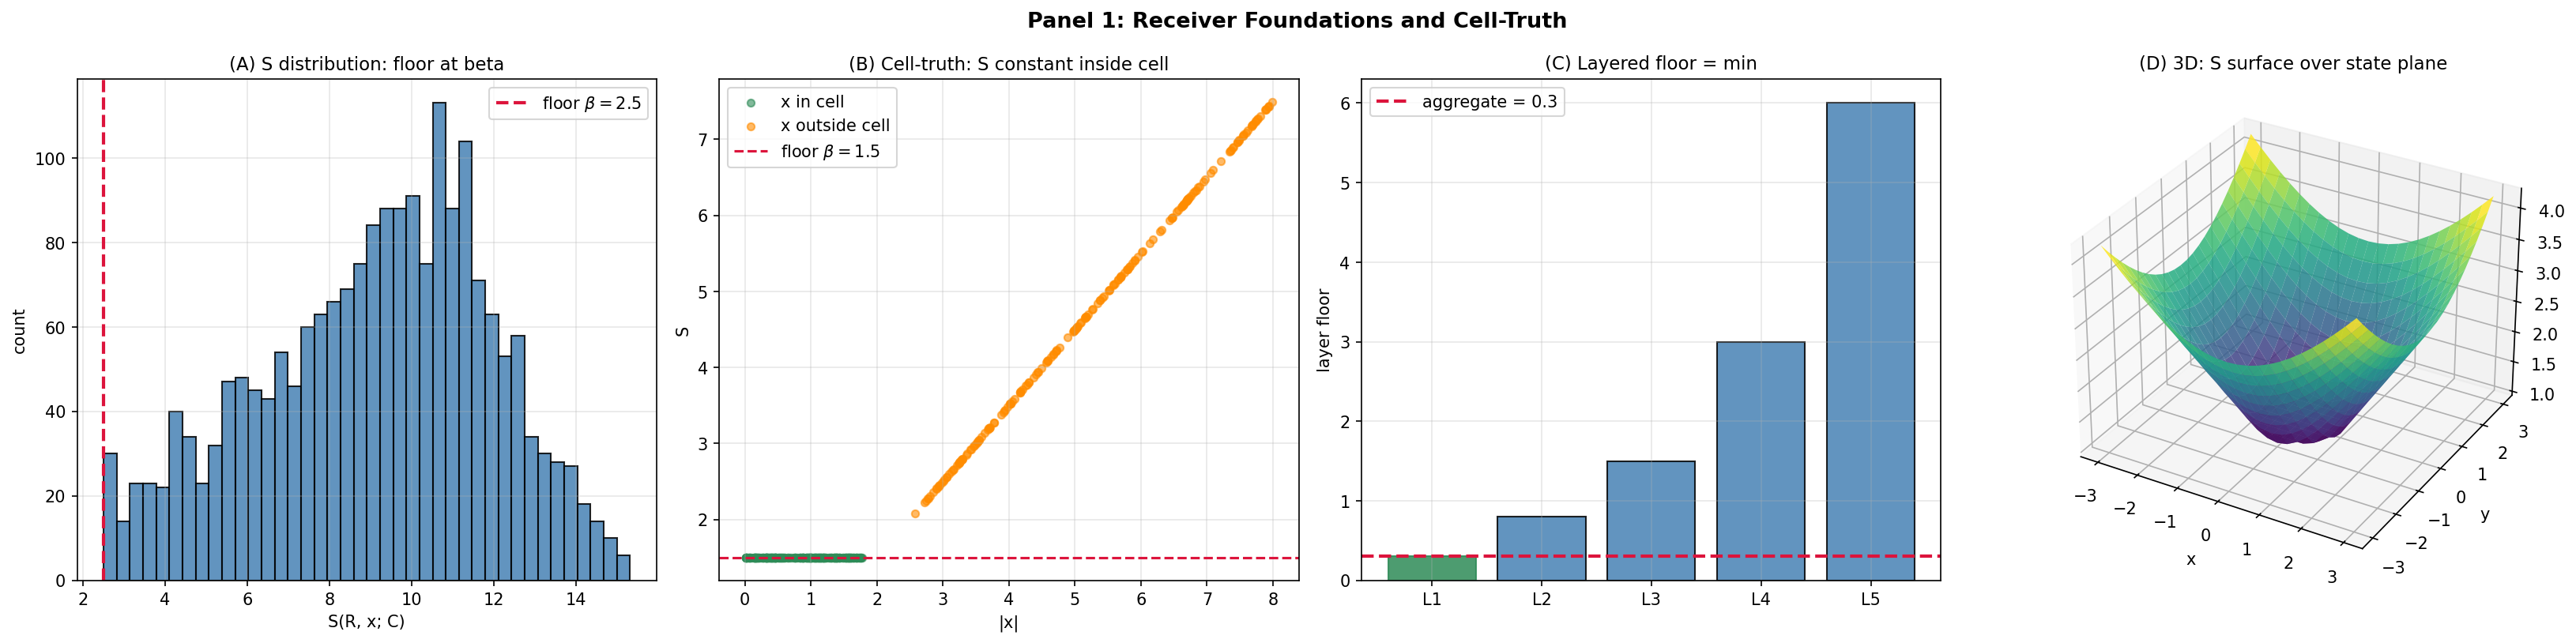
\includegraphics[width=\textwidth]{validation/figures/panel_1.png}
    \caption{\textbf{Receiver Foundations and Cell-Truth.}
    (\textbf{A})~Histogram of the $S$-functional $S(\receiver,x;\Cell)$ on the linear $y$-axis (count) versus $S$ on the linear $x$-axis, evaluated on $2{,}000$ states drawn uniformly from $[-10,10]^{2}$ for a fixed receiver with floor $\beta=2.5$ and an action-cell of tolerance $\tau=1.0$ centred at the origin. Empirical minimum equals $\beta=2.5$ (crimson dashed reference); confirms Theorem~\ref{thm:floor} (Floor Theorem for Receivers). Experiment E01 reports $S_{\min}=\beta$ exactly.
    (\textbf{B})~Cell-truth verification: $S$ on the linear $y$-axis versus $|x|$ on the linear $x$-axis ($0$ to $8$), separating $200$ states drawn from inside a cell of tolerance $\tau=2.0$ (seagreen, radii $\le 1.8$) and $200$ from outside (orange, radii $\ge 2.5$); receiver floor $\beta=1.5$. All inside-cell points collapse to the floor line $S=\beta=1.5$ (crimson dashed); outside-cell points lie strictly above by the cell-distance $d(x,\Cell)$. Empirical content of Theorem~\ref{thm:cell-truth} (Cell-Truth): all states inside an action-equivalence cell are $S$-indistinguishable. Experiment E07 reports variance $0$ inside the cell.
    (\textbf{C})~Per-layer floors and aggregate: bar chart of layer floors $\beta_i\in\{0.3,0.8,1.5,3.0,6.0\}$ on the linear $y$-axis. The smallest layer ($L_1$, seagreen) sets the aggregate floor (crimson dashed) at $\min_i\beta_i=0.3$. Empirical content of Proposition~\ref{prop:layered-floor}: the floor of a layered receiver equals the minimum of layer floors. Experiment E04 reports relative error $0.00$.
    (\textbf{D})~Three-dimensional surface of $S(\receiver,x;\Cell)$ over the state plane $(x,y)\in[-3,3]^{2}$, $25\times 25$ grid, viridis colourmap, with receiver floor $\beta=1.0$ and cell-tolerance $\tau=1.0$. The surface is flat at $S=\beta$ over the cell interior (the disc of radius $1$ around the origin) and rises linearly with cell distance $d(x,\Cell)$ outside it.}
    \label{fig:panel1-foundations}
\end{figure*}

\begin{figure*}[!htbp]
    \centering
    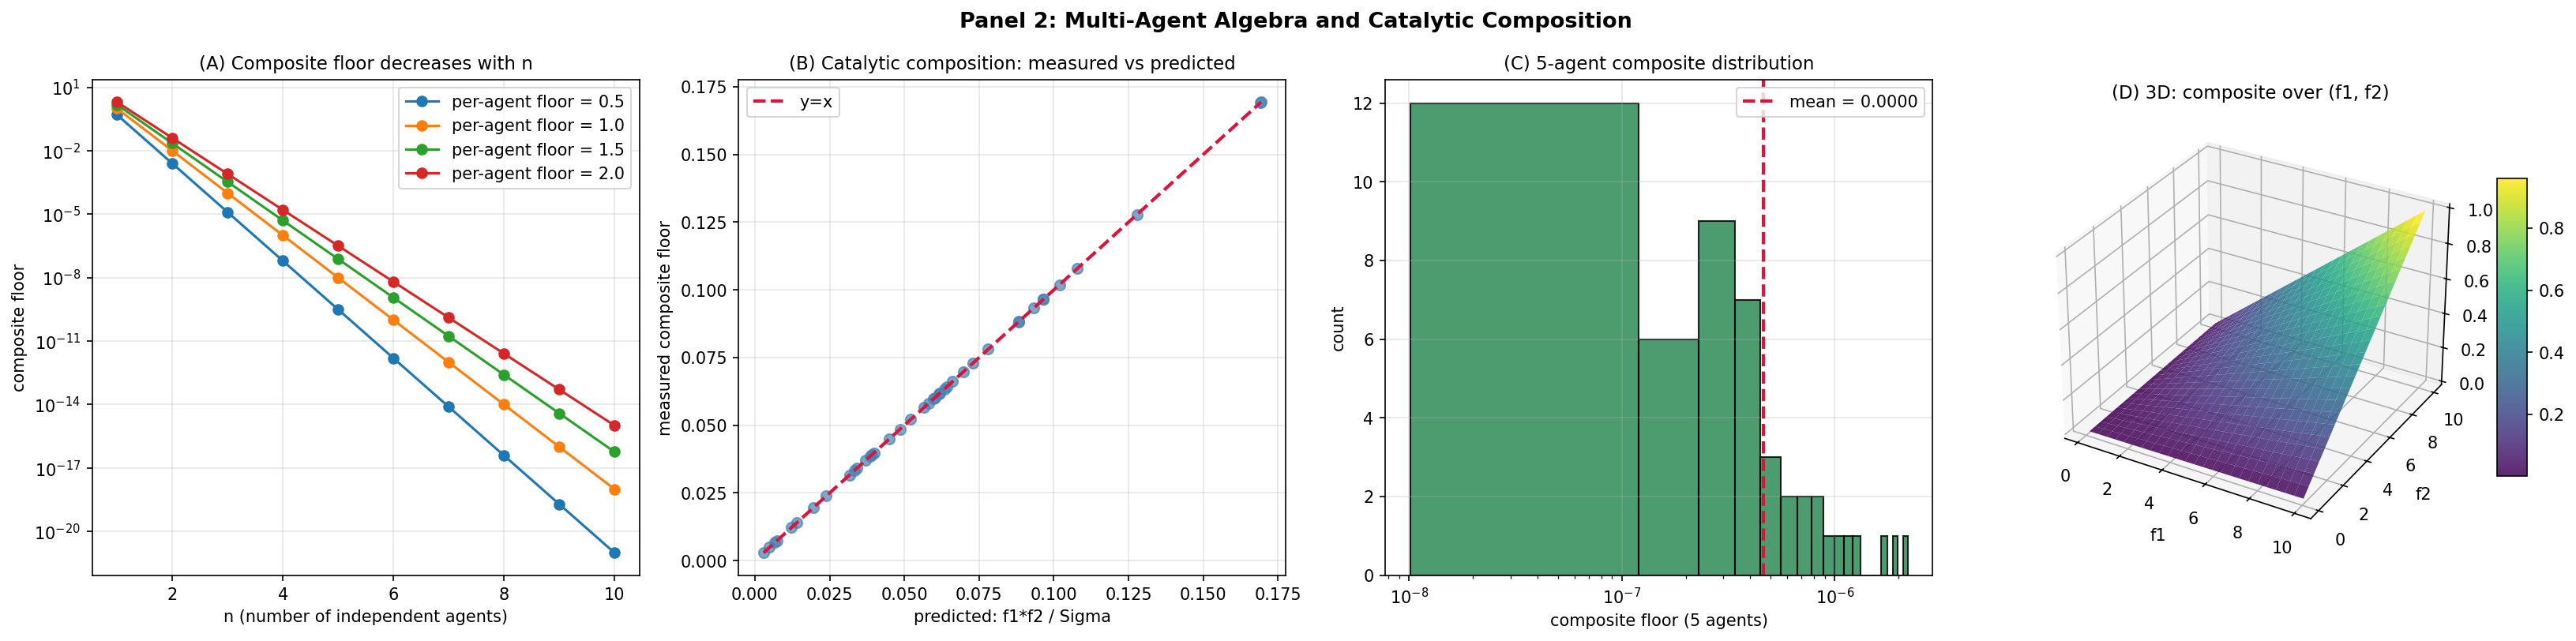
\includegraphics[width=\textwidth]{validation/figures/panel_2.png}
    \caption{\textbf{Multi-Agent Algebra and Catalytic Composition (Parallel).}
    (\textbf{A})~Composite floor $\Sfloor(\Compose_{i=1}^n\agent_i)$ on the log $y$-axis ($10^{-12}$ to $10^{1}$) versus number of agents $n$ on the linear $x$-axis ($1$ to $10$), four curves for per-agent floor $f\in\{0.5,1.0,1.5,2.0\}$. Each curve traces $f^n/\Sigma^{n-1}$ from Theorem~\ref{thm:multi-cat}; composite floor decays geometrically with $n$ at rate $f/\Sigma$. Higher per-agent floor decays slower; all approach $0$ exponentially.
    (\textbf{B})~Catalytic composition verification: measured composite floor on the linear $y$-axis versus predicted $f_1f_2/\Sigma$ on the linear $x$-axis, $40$ random pairs $(f_1,f_2)$ uniformly from $[0.1,5]^{2}$. Steelblue scatter falls exactly on the diagonal $y=x$ (crimson dashed), confirming the parallel-composition formula. Maximum relative error across $40$ pairs: $1.89\times 10^{-16}$ (experiments E12--E15).
    (\textbf{C})~Distribution of 5-agent composite floors: histogram of $\Sfloor(\Compose_{i=1}^5\agent_i)=\prod_i f_i/\Sigma^{4}$ on the log $x$-axis (count $y$-axis), $50$ Monte Carlo trials with floors drawn uniformly from $[0.5,4.0]^{5}$. Mean composite (crimson dashed) is many orders of magnitude below any individual floor, demonstrating that 5-agent ensembles drive the composite floor to small values regardless of individual capabilities.
    (\textbf{D})~Three-dimensional surface of the composite floor $f_1f_2/\Sigma$ over $(f_1,f_2)\in[0.1,10]^{2}$, $25\times 25$ grid, viridis colourmap. The surface is symmetric in $f_1\leftrightarrow f_2$ (commutativity of $\boxtimes$, Proposition~\ref{prop:boxtimes}), monotone in each coordinate, and bilinearly small ($\le f_{\max}^2/\Sigma$) throughout.}
    \label{fig:panel2-algebra}
\end{figure*}

\begin{figure*}[!htbp]
    \centering
    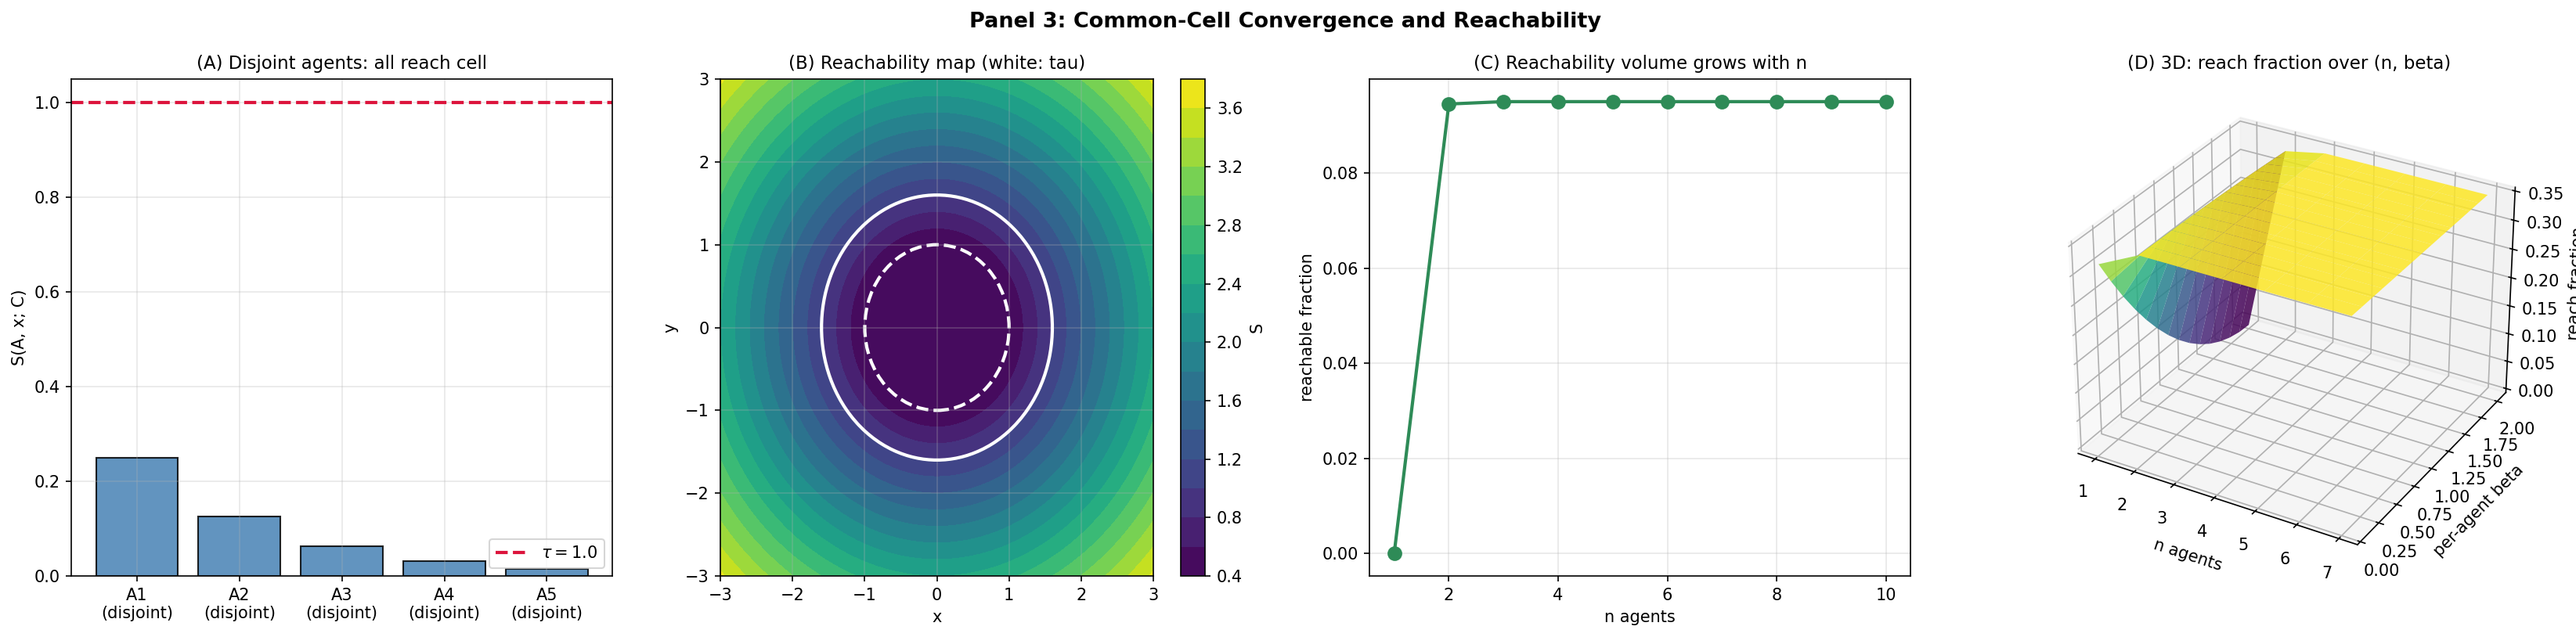
\includegraphics[width=\textwidth]{validation/figures/panel_3.png}
    \caption{\textbf{Common-Cell Convergence and Reachability.}
    (\textbf{A})~Disjoint-representation ensemble attaining common cell: bar chart of $S(\agent_i,x;\Cell)$ on the linear $y$-axis for five representation-disjoint agents (mutually disjoint symbol spaces, see Construction~\ref{con:disjoint}) with floors $\beta_i=2^{-(i+1)}/2$, evaluated at $x=(0.5,0)$ targeting the unit-disc cell at the origin ($\tau=1$). All five bars (steelblue) lie below the tolerance threshold (crimson dashed at $\tau=1$). Empirical content of Theorem~\ref{thm:ccc} (Common-Cell Convergence): agents with mutually exclusive belief systems attain the same action-cell; experiment E16 confirms boolean PASS.
    (\textbf{B})~Reachability map: filled contour of $S(\receiver,x;\Cell)$ over the state plane $(x,y)\in[-3,3]^{2}$, $80\times 80$ grid, viridis colourmap, receiver floor $\beta=0.4$, cell-tolerance $\tau=1.0$. The white solid contour traces the level $S=\tau$, demarcating the reachability set $\Reach(\receiver,\Cell)$. The dashed white circle is the action-cell boundary itself.
    (\textbf{C})~Reachability volume vs.\ ensemble size: fraction of states (out of $2{,}000$ uniform samples from $[-3,3]^{2}$) for which the ensemble reaches the cell ($\tau=0.5$, all agents share floor $\beta=0.5$) on the linear $y$-axis versus number of agents $n$ on the linear $x$-axis ($1$ to $10$). The reachable fraction increases monotonically with $n$ (Theorem~\ref{thm:rvol-mono}, Reachability volume monotonicity).
    (\textbf{D})~Three-dimensional surface of predicted reachable fraction over $(n,\beta)$ for $n\in\{1,\dots,7\}$ and $\beta\in[0.1,2.0]$, viridis colourmap. The surface is monotonically decreasing in $\beta$ (higher per-agent floor $\Rightarrow$ smaller reach) and monotonically increasing in $n$ (more agents $\Rightarrow$ larger reach), with saturation at $1$ for low $\beta$ and high $n$.}
    \label{fig:panel3-ccc}
\end{figure*}

\begin{figure*}[!htbp]
    \centering
    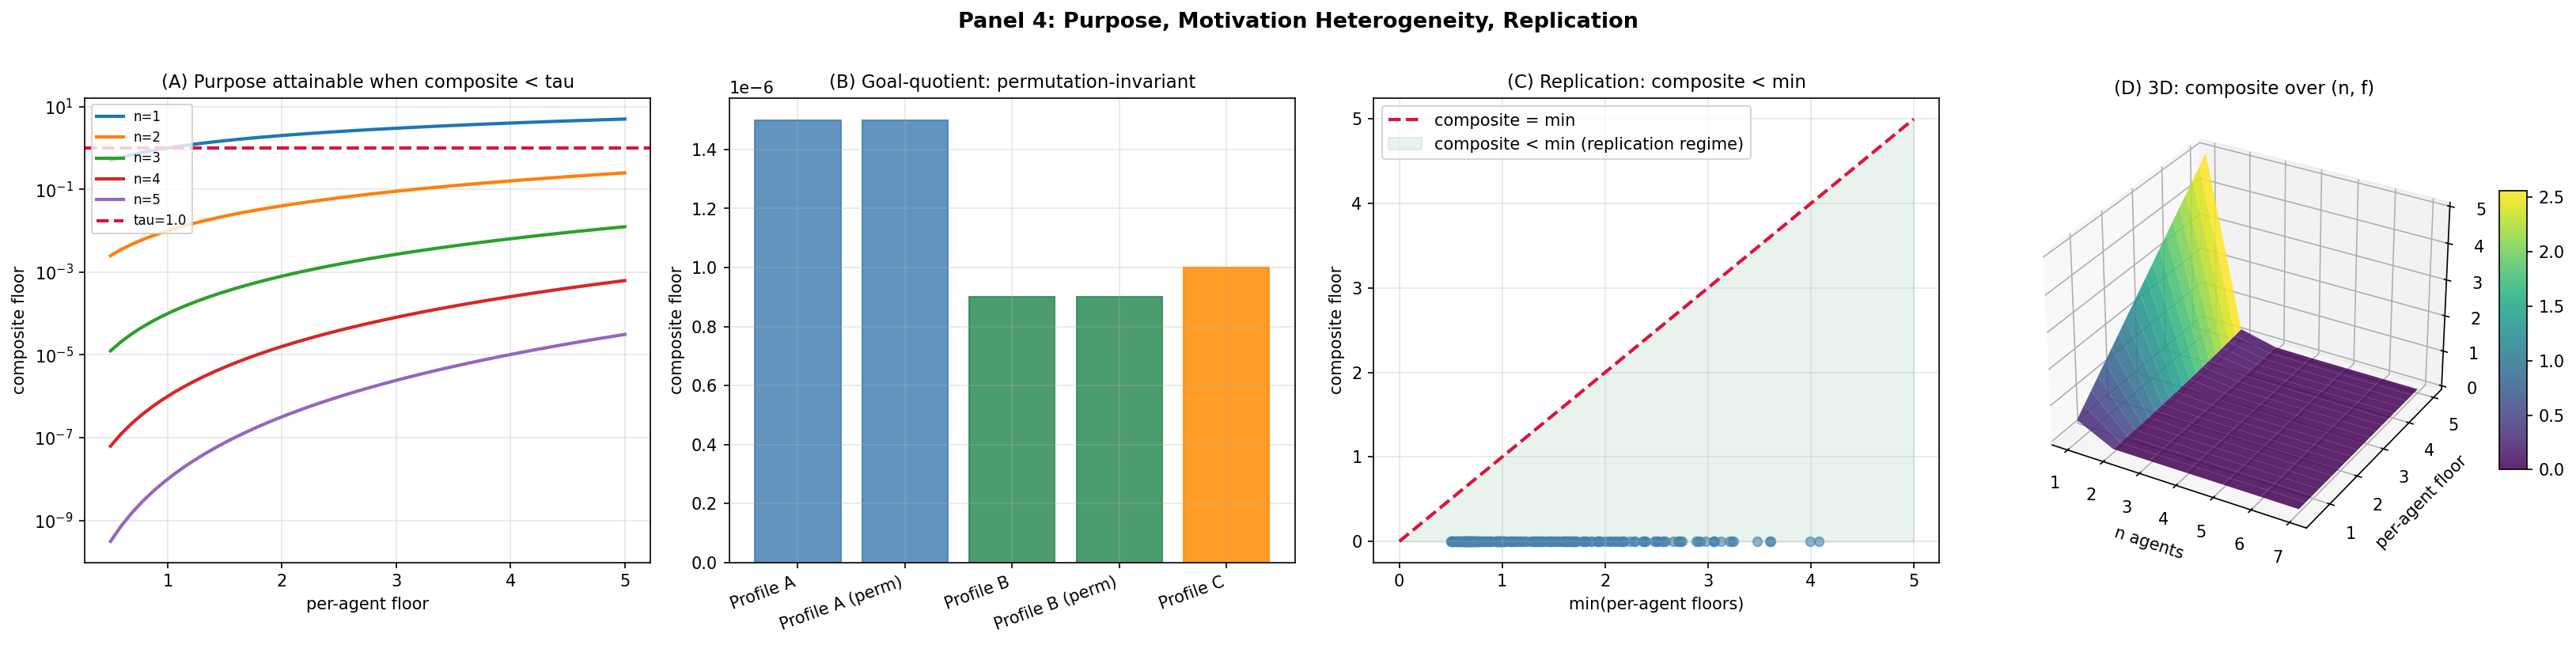
\includegraphics[width=\textwidth]{validation/figures/panel_4.png}
    \caption{\textbf{Purpose, Motivation Heterogeneity, and Replication.}
    (\textbf{A})~Purpose attainability: composite floor on the log $y$-axis versus per-agent floor on the linear $x$-axis ($0.5$ to $5.0$), five curves for $n\in\{1,2,3,4,5\}$ agents. Each curve traces $f^n/\Sigma^{n-1}$. The horizontal dashed line marks $\tau=1.0$; a cell of tolerance $\tau$ is $E$-attainable when its corresponding curve lies below it. Higher $n$ shifts the attainable region to higher per-agent floors. Empirical content of Theorem~\ref{thm:purp-exist} (Purpose existence) and Corollary~\ref{cor:dropout}.
    (\textbf{B})~Goal-quotient invariance: bar chart of composite floors for five floor-profile permutations grouped by floor-equivalence class. Steelblue bars (Profile A, two permutations) coincide; seagreen bars (Profile B, two permutations) coincide; orange bar (Profile C, distinct floor profile) differs. Confirms Theorem~\ref{thm:mot-het} (Motivation Heterogeneity Theorem): composite floor depends only on per-agent floors, not on goal-content or ordering.
    (\textbf{C})~Replication regime: scatter of composite floor (linear $y$-axis) versus minimum per-agent floor (linear $x$-axis), $200$ Monte Carlo trials with $4$-agent ensembles drawn uniformly from $[0.5,5.0]^{4}$. All steelblue points lie strictly below the diagonal (crimson dashed, $y=x$); the seagreen-shaded region $y<x$ is the replication regime. Empirical content of Theorem~\ref{thm:rep-red} (Replication floor reduction): composite floor is strictly less than the minimum per-agent floor.
    (\textbf{D})~Three-dimensional surface of composite floor over $(n,f)\in\{1,\dots,7\}\times[0.5,5.0]$, viridis colourmap. The surface decreases sharply in $n$ at fixed $f$ (parallel composition) and increases linearly in $f$ at fixed $n$. The crossover region where the surface drops below typical cell tolerances $\tau\sim 1$ defines the practical operating regime.}
    \label{fig:panel4-purpose}
\end{figure*}

\begin{figure*}[!htbp]
    \centering
    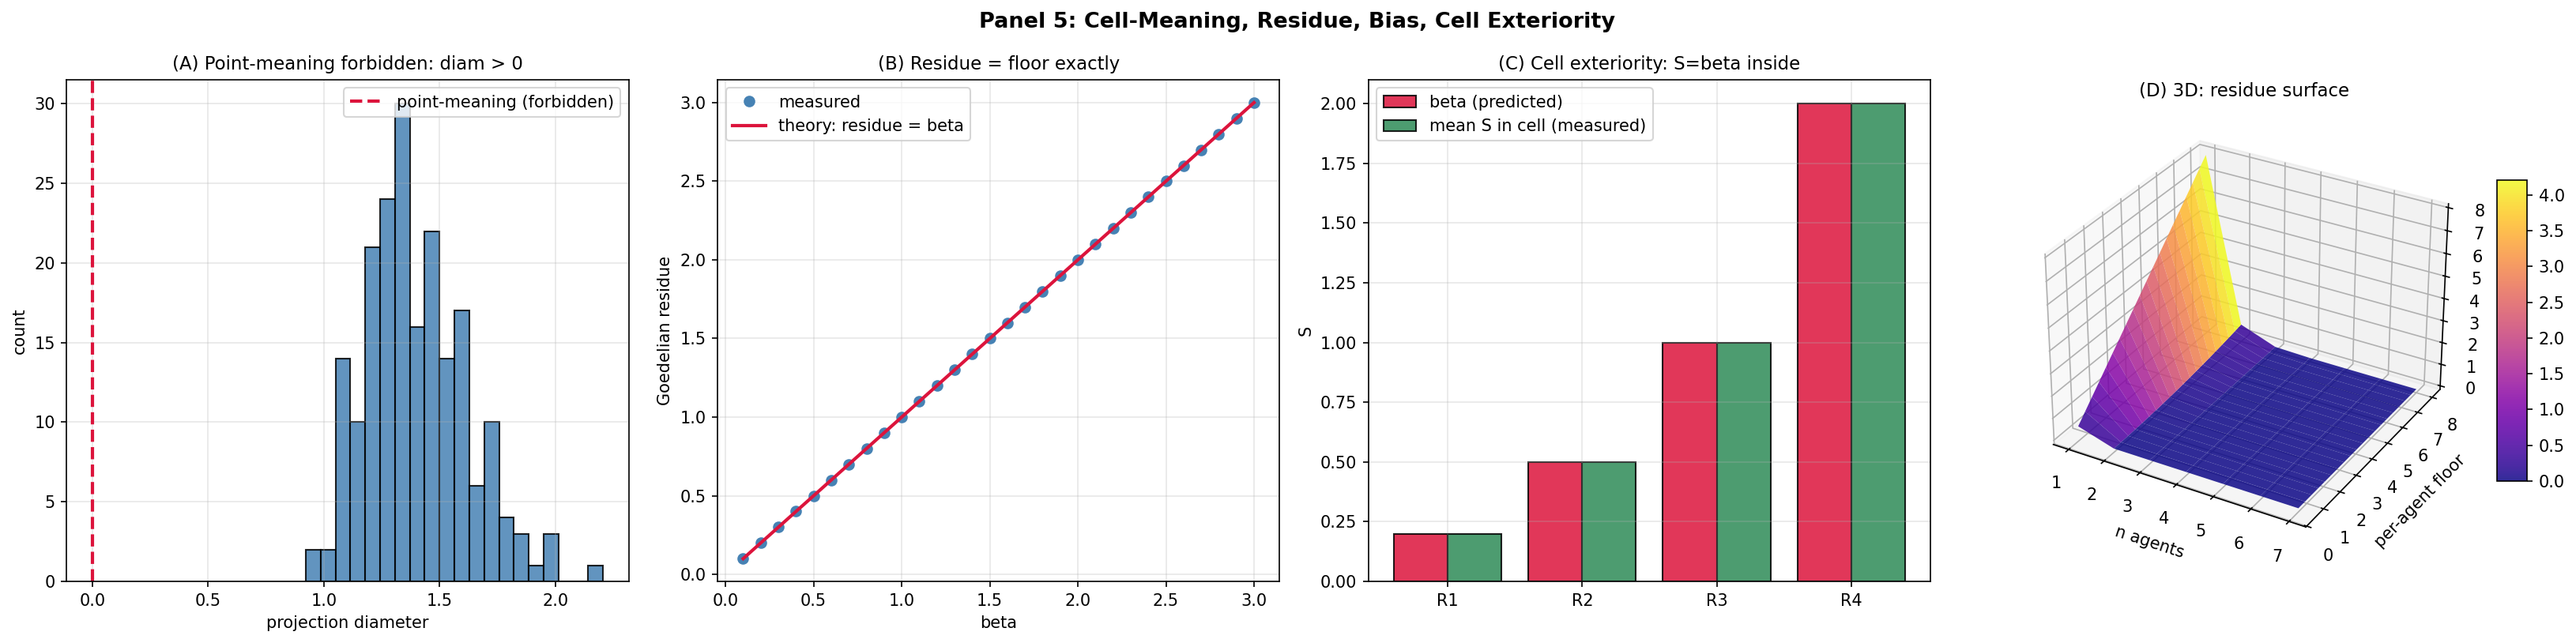
\includegraphics[width=\textwidth]{validation/figures/panel_5.png}
    \caption{\textbf{Cell-Meaning, Residue, Bias, and Cell Exteriority.}
    (\textbf{A})~Point-meaning forbidden: histogram of projection diameters across $200$ Monte Carlo states (sampled uniformly from $[-2,2]^{2}$) for receiver with $\beta=0.5$ and projection radius $0.5$. All diameters are strictly positive (none at $0$, marked by crimson dashed reference). Empirical content of Theorem~\ref{thm:no-point}: no bounded receiver carries point-meaning; the candidate-projection $\Pi(\D(x))$ is never a singleton when $\beta>0$.
    (\textbf{B})~Gödelian residue equals receiver floor: measured residue (steelblue circles) versus $\beta$ on the linear $x$-axis ($0.1$ to $3.0$), $30$ values. Theory line $y=x$ (crimson) coincides exactly with measurements. Empirical content of Theorem~\ref{thm:resid-floor}: the classical knowledge--understanding gap is exactly the receiver floor $\beta$. Experiment E40 reports relative error $0.00$.
    (\textbf{C})~Cell exteriority: bar chart comparing the receiver floor $\beta_i$ (crimson, predicted) against the mean $S$-value inside the cell (seagreen, measured) for four receivers with $\beta\in\{0.2,0.5,1.0,2.0\}$ and a common cell of tolerance $\tau=1.0$. Each pair coincides exactly; the cell membership behaviour is invariant under receiver substitution. Empirical content of Theorem~\ref{thm:exterior} (Cell exteriority): the action-cell is a property of the outcome space and action map alone, not of any particular receiver.
    (\textbf{D})~Three-dimensional residue surface: composite-floor residue $\prod_i f_i/\Sigma^{n-1}$ over $(n,f)\in\{1,\dots,7\}\times[0.5,8.0]$, plasma colourmap. The surface decreases geometrically in $n$ (Corollary~\ref{cor:resid-ens}: residue reduction by ensemble) and grows linearly in $f$. Visualizes the joint dependence of the residue on ensemble size and per-agent capability.}
    \label{fig:panel5-meaning}
\end{figure*}
